\documentclass[aspectratio=169,10pt]{beamer}

% ============================== THEME & FONTS ==============================
\usefonttheme{serif}
\useinnertheme[shadow=true]{rounded}

% ============================== PACKAGES ============================
\usepackage[utf8]{inputenc}
\usepackage[T1]{fontenc}
\usepackage{lmodern}
\usepackage{booktabs}
\usepackage{tabularx}
\usepackage{array}
\usepackage{graphicx}
\usepackage{amsmath,amssymb}
\usepackage{tikz}
\usetikzlibrary{arrows.meta, positioning, shapes.geometric, fit, backgrounds, calc, decorations.pathreplacing}
\usepackage{pgfplots}
\pgfplotsset{compat=1.17}
\usepackage{xcolor}
\usepackage{multirow}
\usepackage{textpos}

% ============================== EXACT PALETTE ==============================
% Extracted directly from reference presentation:
\definecolor{mainblue}{rgb}{0.0, 0.2, 0.4}          % #003366 Deep Navy Blue
\definecolor{blockheaderblue}{rgb}{0.0, 0.3, 0.6}   % #004d99 Medium Dark Blue
\definecolor{blockbodyblue}{rgb}{0.9, 0.93, 0.96}   % #e6edf5 Soft Ice Blue tint
\definecolor{accentblue}{rgb}{0.0, 0.4, 0.8}       % #0066cc Bright Accent Blue
\definecolor{alertbodygray}{rgb}{0.941, 0.941, 0.941} % #f0f0f0 Light Gray
\definecolor{mutedblue}{rgb}{0.35, 0.48, 0.61}      % #597a9c Steel Muted Blue

% Compatibility aliases for diagrams in presentation
\definecolor{navy}{rgb}{0.0, 0.2, 0.4}              % #003366
\definecolor{teal}{rgb}{0.0, 0.4, 0.8}              % #0066cc
\definecolor{orangeaccent}{rgb}{0.0, 0.4, 0.8}      % #0066cc
\definecolor{grayaccent}{rgb}{0.5, 0.5, 0.5}
\definecolor{redaccent}{rgb}{0.8, 0.2, 0.2}

% ============================== BEAMER STYLING ==============================
\setbeamercolor{title}{bg=mainblue,fg=white}
\setbeamercolor{subtitle}{fg=white}
\setbeamercolor{frametitle}{bg=mainblue,fg=white}
\setbeamercolor{structure}{fg=mainblue}
\setbeamercolor{alerted text}{fg=accentblue}

% Blocks: rounded with drop shadow
\setbeamercolor{block title}{bg=blockheaderblue,fg=white}
\setbeamercolor{block body}{bg=blockbodyblue,fg=black}
\setbeamercolor{block title alerted}{bg=accentblue,fg=white}
\setbeamercolor{block body alerted}{bg=alertbodygray,fg=black}
\setbeamercolor{block title example}{bg=accentblue,fg=white}
\setbeamercolor{block body example}{bg=alertbodygray,fg=black}

% Lists: circles and numbers in mainblue
\setbeamertemplate{itemize items}[circle]
\setbeamercolor{itemize item}{fg=mainblue}
\setbeamercolor{itemize subitem}{fg=mainblue}
\setbeamercolor{itemize subsubitem}{fg=mainblue}
\setbeamertemplate{enumerate items}[default]
\setbeamercolor{enumerate item}{fg=mainblue}
\setbeamercolor{enumerate subitem}{fg=mainblue}
\setbeamercolor{enumerate subsubitem}{fg=mainblue}

% Table of Contents: 3D sphere balls
\setbeamertemplate{sections/subsections in toc}[ball]
\setbeamercolor{section number projected}{bg=mainblue,fg=white}

% Frametitle: solid top banner
\setbeamertemplate{frametitle}{%
  \nointerlineskip%
  \begin{beamercolorbox}[wd=\paperwidth,ht=25pt,dp=6pt,leftskip=8.5pt]{frametitle}%
    \usebeamerfont{frametitle}\insertframetitle\par%
  \end{beamercolorbox}%
}

% Author separator: line break to stack authors cleanly like reference slide 1
\makeatletter
\def\beamer@andtitle{\\[4pt]}
\makeatother

% Title page: rounded shadow box for title/subtitle, authors and details centered below
\setbeamertemplate{title page}{%
  \vbox{}
  \vskip 1.2em%
  \begin{beamercolorbox}[sep=8pt,center,rounded=true,shadow=true]{title}%
    {\usebeamerfont{title}\bfseries\inserttitle\par}%
    \ifx\insertsubtitle\@empty\else%
      \vskip 0.4em%
      {\usebeamerfont{subtitle}\insertsubtitle\par}%
    \fi%
  \end{beamercolorbox}%
  \vskip 1.3em%
  \begin{centering}%
    {\usebeamerfont{author}\insertauthor\par}%
    \vskip 1.1em%
    {\usebeamerfont{institute}\footnotesize\insertinstitute\par}%
    \vskip 1.1em%
    {\usebeamerfont{date}\insertdate\par}%
  \end{centering}%
  \vfill%
}

% Footline: minimal, only slide numbers at bottom right
\setbeamertemplate{navigation symbols}{}
\setbeamertemplate{footline}{%
  \hfill%
  \usebeamercolor[fg]{page number in head/foot}%
  \usebeamerfont{page number in head/foot}%
  \tiny\insertframenumber{} / \inserttotalframenumber%
  \hspace*{8.5pt}\vskip5pt%
}

% Bibliography styling matching reference
\setbeamertemplate{bibliography item}[article]
\setbeamercolor{bibliography entry author}{fg=mainblue}
\setbeamercolor{bibliography entry title}{fg=black}
\setbeamercolor{bibliography entry location}{fg=mutedblue}
\setbeamercolor{bibliography entry note}{fg=mutedblue}

% ============================== INFO ================================
\title{Robust and Generalizable Decision-Making for CAVs at Unsignalized Intersections}
\subtitle{A Deep Reinforcement Learning Approach — Reproduction, Benchmarking \& Path to Generalization}
\author{Mahmudul Hasan (220041231) \and Ishmam Tahmid (220041259) \and Farhan Tahsin Khan (220041229)}
\institute{
    CSE 4610: Design Project \\[2pt]
    \small Supervisors: Ashraful Alam Khan \quad \& \quad Tanjila Alam Sathi \\
    \small Course Coordinator: Dr.\ Md.\ Azam Hossain
}
\date{September 14, 2026}

\begin{document}

% ============================== TITLE ==============================
\begin{frame}
    \titlepage
\end{frame}

\begin{frame}{Outline}
    \tableofcontents
\end{frame}

% =====================================================================
\section{Introduction}
% =====================================================================

\begin{frame}{Introduction: The Problem}
    \begin{columns}[T]
        \begin{column}{0.48\textwidth}
            \textbf{The Problem with Traffic Lights}
            \begin{itemize}
                \item Fixed or semi-adaptive timing $\rightarrow$ vehicles stop even when the road is clear
                \item Control happens at the \alert{lane-group} level, not the individual vehicle
                \item Wastes fuel, time, and causes unnecessary idling / emissions
            \end{itemize}
        \end{column}
        \begin{column}{0.48\textwidth}
            \textbf{The Scale of the Problem}
            \begin{itemize}
                \item $\sim$36\% of all crashes are intersection-related \cite{zhong2021survey}
                \item Intersection crashes: \$371B societal cost (US, 2010) \cite{zhong2021survey}
                \item Over 40\% of collisions in EU/US occur at intersections \cite{gholamhosseinian2022survey}
            \end{itemize}
        \end{column}
    \end{columns}
    \vspace{8pt}
    \begin{alertblock}{Core Issue}
        Signalized intersections cause major traffic bottlenecks, while unsignalized crossings face severe collision risks due to blind-spot occlusions and uncertain multi-agent interactions.
    \end{alertblock}
\end{frame}

\begin{frame}{Introduction: Motivation}
    \begin{columns}[T]
        \begin{column}{0.48\textwidth}
            \textbf{Why CAV, Not Just AV?}
            \begin{itemize}
                \item \textbf{Autonomous Vehicle (AV)}: Relies purely on onboard sensing (camera, lidar, radar); blind to occlusions and other drivers' intent
                \item \textbf{Connected \& Automated Vehicle (CAV)}: V2X communication shares position, speed, and \alert{intent} beyond line-of-sight
            \end{itemize}
        \end{column}
        \begin{column}{0.48\textwidth}
            \textbf{Signal-Free AIM \& Deep RL}
            \begin{itemize}
                \item \textbf{Autonomous Intersection Management}: Signal-free coordination enables continuous vehicle throughput without stopping
                \item \textbf{Deep Reinforcement Learning}: Learns adaptive, continuous go/yield negotiation under dense, stochastic traffic
            \end{itemize}
        \end{column}
    \end{columns}
    \vspace{8pt}
    \begin{alertblock}{Key Idea}
        V2X lets a CAV reason about \emph{what other vehicles intend to do}, not just where they are — this is exactly the gap our RL state design (task-intent feature $\mu_a$) is built to exploit.
    \end{alertblock}
\end{frame}

% (Part of Introduction)

\begin{frame}{Core Challenge}
    \begin{center}
        \Large How can an autonomous ego vehicle decide, at every timestep, whether to \alert{go} or \alert{yield} among randomly-behaving vehicles at an unsignalized intersection --- safely, efficiently, and reliably?
    \end{center}
    \vspace{10pt}
    \begin{itemize}
        \item Multiple simultaneous, uncertain decisions among interacting vehicles
        \item No shared reservation protocol; right-of-way must be inferred, not commanded
        \item Must remain reliable across traffic density, driving styles, and geometries
    \end{itemize}
\end{frame}

\begin{frame}{Key Objectives}
    \begin{columns}
        \begin{column}{0.32\textwidth}
            \begin{block}{Safety}
                \centering
                Zero (or near-zero) collisions across randomized turning tasks
            \end{block}
        \end{column}
        \begin{column}{0.32\textwidth}
            \begin{block}{Efficiency}
                \centering
                Minimize crossing / travel time, maximize throughput speed
            \end{block}
        \end{column}
        \begin{column}{0.32\textwidth}
            \begin{block}{Robustness}
                \centering
                Stable performance across traffic densities \emph{and}, eventually, geometries
            \end{block}
        \end{column}
    \end{columns}
\end{frame}

% =====================================================================
\section{Related Work}
% =====================================================================

\begin{frame}{Landscape of Coordination Strategies}
    \small
    \begin{columns}[T]
        \begin{column}{0.5\textwidth}
            \textbf{By architecture}
            \begin{itemize}
                \item \textbf{Centralized}: reservation scheme, optimization-based
                \item \textbf{Decentralized}: virtual vehicle/platooning, fuzzy logic, invariant sets, local MPC
            \end{itemize}
            \textbf{By scheduling policy}
            \begin{itemize}
                \item FCFS $\;\to\;$ Heuristic $\;\to\;$ Optimization-based
            \end{itemize}
        \end{column}
        \begin{column}{0.5\textwidth}
            \textbf{By intersection modeling}
            \begin{itemize}
                \item Spatio-Temporal Reservation: Intersection-Based / Tile-Based
                \item Trajectory Planning: Conflict-Point-Based / Vehicle-Based
            \end{itemize}
            \textbf{By goal}
            \begin{itemize}
                \item Safety, Efficiency, Environment, Infotainment
            \end{itemize}
        \end{column}
    \end{columns}
    \vspace{6pt}
    \begin{center}
    \footnotesize
    \begin{tabular}{lll}
        \toprule
        \textbf{Axis} & \textbf{Most popular} & \textbf{Runner-up} \\
        \midrule
        Goal & Safety + Efficiency (37\%) & Safety alone (26\%) \\
        Architecture & V2V (159 papers) & V2I (119 papers) \\
        Scheduling & Optimization (277 papers) & Heuristic (20 papers) \\
        Modeling & Trajectory Planning & Spatio-Temporal Reservation \\
        \bottomrule
    \end{tabular}
    \end{center}
    \tiny Source: \cite{gholamhosseinian2022survey} (379-paper systematic review); context also from \cite{riostorres2017survey, zhong2021survey}.
\end{frame}

\begin{frame}{Approach Families: Strengths \& Limitations}
    \small
    \begin{table}
    \begin{tabularx}{\textwidth}{@{}l X X@{}}
        \toprule
        \textbf{Approach} & \textbf{Strength} & \textbf{Limitation} \\
        \midrule
        Heuristic / Rule-based (FCFS, TTC) & Simple, transparent, cheap & Rigid; degrades sharply as traffic complexity grows \\
        Classical Optimization (MPC, reservation) & Best-possible solution given the model & Computationally heavy; mostly simulation-only \\
        RL / Deep RL & Adapts to uncertainty; learns implicit right-of-way & Data-hungry; no formal safety guarantee; harder to interpret \\
        \bottomrule
    \end{tabularx}
    \end{table}
    \vspace{4pt}
    \begin{alertblock}{Why DRL for this project}
        Unsignalized, randomized-task intersections are exactly where fixed heuristics break down and full optimization is too slow for real-time control --- DRL trades a formal guarantee for adaptability, which is the core trade-off this project investigates.
    \end{alertblock}
\end{frame}

\begin{frame}{RL Literature Thread I: Single-Ego Decision Making}
    \scriptsize
    \begin{table}
    \begin{tabularx}{\textwidth}{@{}l X X X@{}}
        \toprule
        \textbf{Paper} & \textbf{Idea} & \textbf{Architecture} & \textbf{Key finding} \\
        \midrule
        Isele et al.\ 2018 \cite{isele2018navigating} & DQN vs.\ TTC heuristic + active-sensing ``creeping'' under occlusion & Single-agent, no comm. & 28\% faster crossing, $<$1\% collisions vs.\ TTC \\
        Wu et al.\ 2019 DCL-AIM \cite{wu2019dclaim} & Decentralized coordination Q-learning & Multi-agent, sparse comm. & Beats FCFS/LQF/Webster signal at every traffic rate \\
        Kai et al.\ 2020 \cite{kai2020multitask} & One shared policy for 3 maneuvers via task vector & Single-agent & Matches/beats 3 separate DQNs \\
        Shu et al.\ 2022 \cite{shu2022drivingtasks} & Transfers weights between per-maneuver networks & Single-agent & Same-task transfer up to 100\%, cross-task $>$70\% \\
        \bottomrule
    \end{tabularx}
    \end{table}
    \vspace{4pt}
    \textbf{Convergent finding:} straight/right-turn is easy (high right-of-way); \alert{left-turn is consistently hard} --- confirmed independently by multiple papers.
\end{frame}

\begin{frame}{RL Literature Thread II: Graph Representations \& Cooperative AIM}
    \scriptsize
    \begin{table}
    \begin{tabularx}{\textwidth}{@{}l X X@{}}
        \toprule
        \textbf{Paper} & \textbf{Contribution} & \textbf{Setting} \\
        \midrule
        Chen et al.\ 2025 \cite{chen2025unified} & Scenario-agnostic ``lane-gap'' representation + PPO + CILQR & Single-ego, multi-scenario (93--97\% success) \\
        Schier et al.\ 2023 \cite{schier2023deep} & Heterogeneous vehicle+road graph, learned edges (GATv2 + Dueling DQN) & Single-ego; edges predict right-of-way at 99.5\% acc. \\
        Klimke et al.\ 2022 \cite{klimke2022enhanced} & Edge-augmented RGCN + TD3, centrally controls \emph{all} vehicles & \alert{True cooperative AIM}; beats FIFO/eFIFO/traffic-light \\
        Huamán Reyna et al.\ 2026 \cite{huamanreyna2026review} & Survey of 53 papers, single- vs.\ multi-scenario DM & Hybrid methods score best on adaptability + safety \\
        \bottomrule
    \end{tabularx}
    \end{table}
    \vspace{6pt}
    \begin{block}{Positioning of our project}
        Like Kai et al.\ and Xiao et al., we study \emph{single-ego} decision-making with a \emph{multi-task} state --- not centralized cooperative AIM (Klimke et al.) --- which keeps the problem tractable for a design-project scope while remaining directly comparable to the reproduction target.
    \end{block}
\end{frame}

% =====================================================================
\section{Methodology}
% =====================================================================

\begin{frame}{Methodology}
    % [Template slide: Add Methodology overview content here]
\end{frame}

\begin{frame}{Reproduction Target: Xiao et al.\ (2024, IEEE T-VT)}
    \textbf{``Decision-Making for Autonomous Vehicles in Random Task Scenarios at Unsignalized Intersection Using Deep Reinforcement Learning''} \cite{xiao2024decision}
    \vspace{6pt}
    \begin{columns}[T]
        \begin{column}{0.55\textwidth}
            \textbf{Three contributions}
            \begin{enumerate}
                \item \textbf{Mix-Attention Network} replacing the plain MLP in SAC
                \item \textbf{Task-intent state variable} $\mu_a$: encodes maneuver progress (left / straight / right)
                \item \textbf{Segmented replay buffer}: separates (reach-goal, collision) experience from (neither) experience
            \end{enumerate}
        \end{column}
        \begin{column}{0.45\textwidth}
            \begin{block}{Setting}
                4-way, single-lane, unsignalized intersection; random driving task per episode; SUMO-free custom \texttt{highway-env} simulator; SAC (discrete actions), 50{,}000 training episodes
            \end{block}
        \end{column}
    \end{columns}
\end{frame}

\begin{frame}{Disclaimer: What This Project Is (and Isn't)}
    \begin{alertblock}{This is a reproduction \& benchmarking study --- not our primary contribution}
        The goal is to build a working training pipeline, deeply understand the environment and algorithm, and use that foundation to propose a novel direction (generalization) for future work.
    \end{alertblock}
    \vspace{6pt}
    \textbf{Acknowledged limitations}
    \begin{itemize}
        \item The original paper's source code was \alert{not publicly released}
        \item Several implementation details (exact reward shaping constants, some hyperparameters, buffer split schedule details) were only partially specified
        \item Our reproduction is therefore \alert{not a byte-for-byte replica} --- but it is faithful to every specification the paper gives explicitly
    \end{itemize}
\end{frame}

\begin{frame}{Current Progress}
    \begin{columns}[T]
        \begin{column}{0.5\textwidth}
            \textbf{Completed}
            \begin{itemize}
                \item Milestone 1: single-agent ring-road stabilization (PPO) --- pipeline sanity check
                \item Milestone 2: PPO baseline on the 4-way intersection, \textbf{2 of 8} paper configurations (Original vs.\ Config B)
                \item Milestone 3: \textbf{exact} algorithm match --- Discrete SAC, 50k episodes, full state/reward/network match
            \end{itemize}
        \end{column}
        \begin{column}{0.5\textwidth}
            \textbf{Remaining directions}
            \begin{itemize}
                \item Remaining 6 of 8 original configurations
                \item Mix-Attention network ablation (ours currently uses the plain MLP backbone from the paper's baseline)
                \item Segmented replay buffer improvement (Improvement C in the paper)
            \end{itemize}
        \end{column}
    \end{columns}
\end{frame}

\begin{frame}{Research Progression: Three Milestones}
    \centering
    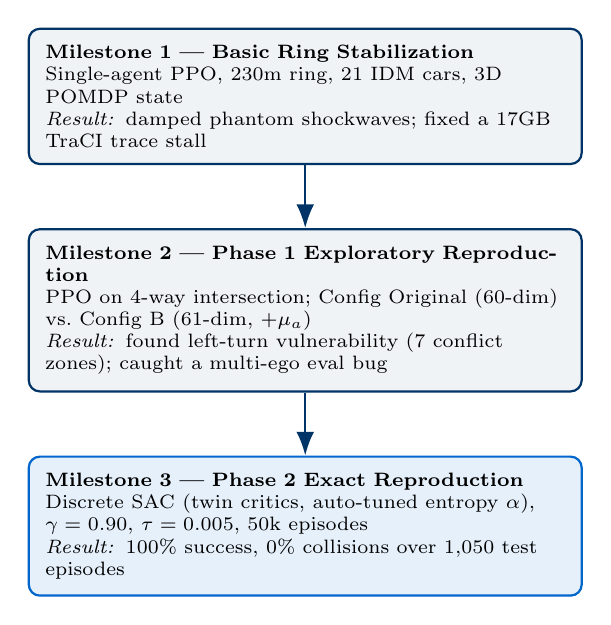
\begin{tikzpicture}[
        node distance=8mm and 14mm,
        every node/.style={font=\scriptsize},
        box/.style={draw=navy, thick, rounded corners, fill=navy!6, text width=6.6cm, align=left, inner sep=6pt},
        arrowstyle/.style={-{Latex[length=3mm]}, thick, navy}
    ]
        \node[box] (m1) {
            \textbf{Milestone 1 --- Basic Ring Stabilization}\\
            Single-agent PPO, 230m ring, 21 IDM cars, 3D POMDP state\\
            \textit{Result:} damped phantom shockwaves; fixed a 17GB TraCI trace stall
        };
        \node[box, below=of m1] (m2) {
            \textbf{Milestone 2 --- Phase 1 Exploratory Reproduction}\\
            PPO on 4-way intersection; Config Original (60-dim) vs.\ Config B (61-dim, $+\mu_a$)\\
            \textit{Result:} found left-turn vulnerability (7 conflict zones); caught a multi-ego eval bug
        };
        \node[box, below=of m2, fill=teal!10, draw=teal] (m3) {
            \textbf{Milestone 3 --- Phase 2 Exact Reproduction}\\
            Discrete SAC (twin critics, auto-tuned entropy $\alpha$), $\gamma=0.90$, $\tau=0.005$, 50k episodes\\
            \textit{Result:} 100\% success, 0\% collisions over 1{,}050 test episodes
        };
        \draw[arrowstyle] (m1) -- (m2);
        \draw[arrowstyle] (m2) -- (m3);
    \end{tikzpicture}
\end{frame}

% (Part of Methodology)

\begin{frame}{State Space}
    \small
    For AEV $a$ and up to 9 nearest surrounding vehicles $i$ (48m detection radius):
    \[
        S = (S_a,\, S_i), \qquad
        S_a = (p_a, x_a, y_a, v_{x_a}, v_{y_a}, \varphi_a,\, \mu_a), \qquad
        S_i = (p_i, \Delta x_i, \Delta y_i, \Delta v_{x_i}, \Delta v_{y_i}, \varphi_i, 0)
    \]
    \begin{itemize}
        \item $p$: existence flag; non-existent vehicles are zero-filled
        \item $\mu_a$: \alert{task-intent feature} --- angular/positional progress toward the exit, distinguishing left / straight / right
        \item Total: $6 + 9\times 6 = 60$-dim (Original) or $61$-dim (Config B, with $\mu_a$)
    \end{itemize}
    \vspace{4pt}
    \begin{block}{Why $\mu_a$ matters}
        The AEV knows its \emph{own} intent but not others' --- $\mu_a$ lets the policy condition its speed profile on its own upcoming maneuver curvature without collapsing to a memorized one-hot per task.
    \end{block}
\end{frame}

\begin{frame}{Action Space \& Reward Function}
    \begin{columns}[T]
        \begin{column}{0.42\textwidth}
            \textbf{Action space} (discrete, 3 values)
            \[
                A = \{\text{accelerate}, \text{idle}, \text{decelerate}\}
            \]
            Mapped to target speed via a P-controller:
            \[
                a = K_{P,A}(v_{tar} - v), \quad K_{P,A}=5
            \]
            Lateral control (steering) is handled separately by a fixed PD lane-tracking controller --- \alert{RL only controls longitudinal speed}.
        \end{column}
        \begin{column}{0.58\textwidth}
            \textbf{Reward function}
            \[
                R = \begin{cases}
                    +30 & \text{reach destination} \\
                    -120 & \text{collision occurs} \\
                    +0.1 & \text{reach target speed}
                \end{cases}
            \]
            \begin{itemize}
                \item Sparse terminal terms (safety + task completion)
                \item Small dense term rewards efficient cruising
                \item Large collision penalty $\gg$ arrival reward $\to$ safety-dominant shaping
            \end{itemize}
        \end{column}
    \end{columns}
\end{frame}

\begin{frame}{System Pipeline}
    \centering
    \resizebox{\textwidth}{!}{%
    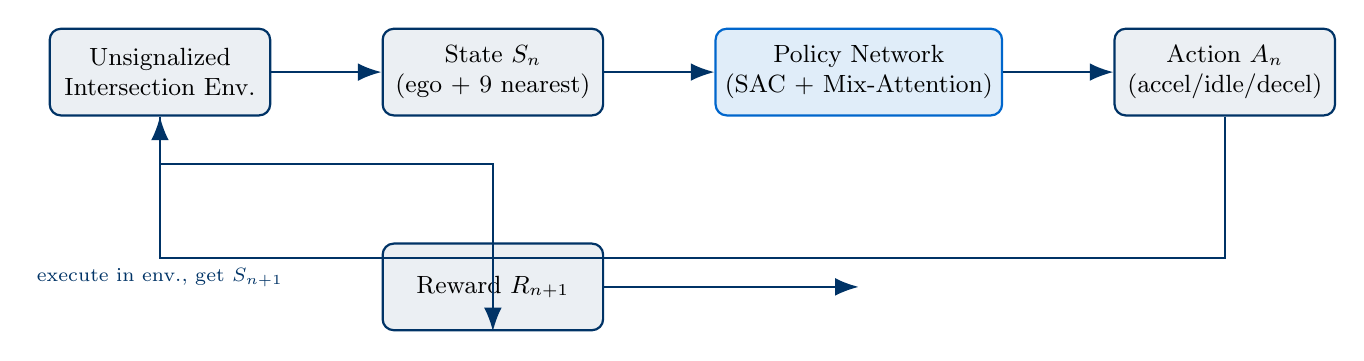
\begin{tikzpicture}[
        node distance=9mm,
        every node/.style={font=\small},
        block/.style={draw=navy, thick, rounded corners, fill=navy!8, minimum height=1.1cm, minimum width=2.8cm, align=center},
        arrowstyle/.style={-{Latex[length=3mm]}, thick, navy}
    ]
        \node[block] (env) {Unsignalized\\Intersection Env.};
        \node[block, right=14mm of env] (state) {State $S_n$\\(ego + 9 nearest)};
        \node[block, right=14mm of state, fill=teal!12, draw=teal] (policy) {Policy Network\\(SAC + Mix-Attention)};
        \node[block, right=14mm of policy] (action) {Action $A_n$\\(accel/idle/decel)};
        \node[block, below=16mm of state, minimum width=2.8cm] (reward) {Reward $R_{n+1}$};

        \draw[arrowstyle] (env) -- (state);
        \draw[arrowstyle] (state) -- (policy);
        \draw[arrowstyle] (policy) -- (action);
        \draw[arrowstyle] (action.south) |- ($(action.south)+(0,-18mm)$) -| (env.south)
            node[midway, below, font=\scriptsize] {execute in env., get $S_{n+1}$};
        \draw[arrowstyle] (env.south) -- ++(0,-6mm) -| (reward.south);
        \draw[arrowstyle] (reward) -- (policy.south |- reward);
    \end{tikzpicture}%
    }
    \vspace{10pt}
    \small Simulation frequency 15\,Hz, policy (decision) frequency 1\,Hz, episode duration 25\,s --- exactly matching Xiao et al.\ \cite{xiao2024decision}.
\end{frame}

\begin{frame}{Discrete Soft Actor-Critic (Discrete SAC)}
    \small
    \begin{columns}[T]
        \begin{column}{0.5\textwidth}
            \textbf{Why SAC over PPO here}
            \begin{itemize}
                \item Off-policy $\to$ high sample efficiency (crucial with a 150k-transition replay buffer)
                \item Maximum-entropy objective encourages broad exploration, avoids premature convergence in a highly randomized task space
                \item Auto-tuned temperature $\alpha$ removes a fragile hand-tuned hyperparameter
            \end{itemize}
        \end{column}
        \begin{column}{0.5\textwidth}
            \[
                \pi^{*} = \arg\max_\pi \sum_{n} \mathbb{E}\big[\gamma^n (R_n + \alpha \mathcal{H}(\pi(\cdot|S_n)))\big]
            \]
            \begin{itemize}
                \item Twin Q-critics (clipped double-Q) reduce overestimation bias
                \item Discrete action variant: policy outputs a categorical distribution via softmax, no reparameterization trick needed
            \end{itemize}
        \end{column}
    \end{columns}
\end{frame}

% =====================================================================
\section{Implementation}
% =====================================================================

\begin{frame}{Implementation}
    % [Template slide: Add Implementation details/architecture here]
\end{frame}

\begin{frame}{Simulation \& Training Setup}
    \scriptsize
    \begin{table}
    \begin{tabularx}{\textwidth}{@{}l X X X X@{}}
        \toprule
         & \textbf{Project 1: Basic Ring} & \textbf{Project 2: Phase 1} & \textbf{Project 3: Phase 2} & \textbf{Paper (Xiao et al.)} \\
        \midrule
        Scenario & 230m single-lane ring & 4-way intersection & 4-way intersection & 4-way intersection \\
        Sim.\ engine & Flow + SUMO & Flow + SUMO & \texttt{highway-env} & \texttt{highway-env} \\
        Algorithm & PPO (RLlib) & PPO (RLlib) & \textbf{Discrete SAC} & \textbf{Discrete SAC} \\
        Network & Actor-Critic MLP & $[32,32,32]$ MLP & $[256,256,64,3]$ MLP & $[256,256,64,3]$ MLP \\
        Obs.\ space & 3-dim POMDP & 60 / 61-dim & 60 / 61-dim & 60 / 61-dim \\
        Action space & Continuous, $[-1,1]\,\mathrm{m/s^2}$ & Discrete(3) & Discrete(3) & Discrete(3) \\
        Training budget & 123 iters ($\sim$7.4M steps) & 2.5k / 9.36k iters & \textbf{50{,}000 episodes} & \textbf{50{,}000 episodes} \\
        \bottomrule
    \end{tabularx}
    \end{table}
    \vspace{4pt}
    \centering \small $\gamma = 0.90$, $\tau = 0.005$ (soft update), replay capacity $=150{,}000$, batch size $=1024$ --- matched to the paper for Project 3.
\end{frame}

\begin{frame}{Systems Engineering: Hardware Scaling Challenge}
    \begin{columns}[T]
        \begin{column}{0.45\textwidth}
            \textbf{Problem discovered}
            \begin{itemize}
                \item Intel hybrid-CPU (P-core / E-core) architectures suffer OpenMP thread-sync stalls during SUMO/SAC training
                \item Default scheduling let threads bounce across core types
            \end{itemize}
            \textbf{Fix}
            \begin{itemize}
                \item Pin training threads to physical performance cores only (\texttt{taskset} affinity 0,2,4,6)
            \end{itemize}
        \end{column}
        \begin{column}{0.55\textwidth}
            \centering
            
\includegraphics[width=\linewidth]{img/pcore_affinity_chart.png}
        \end{column}
    \end{columns}
    \vspace{2pt}
    \centering \footnotesize $46 \to 160$ episodes/min ($\sim$3.5$\times$); total training time cut from 18h to 6.9h.
\end{frame}

% =====================================================================
\section{Experimental Results}
% =====================================================================

\begin{frame}{Result 1: Success \& Collision Rate}
    \centering
    
\includegraphics[width=0.62\linewidth]{img/success_collision_chart.png}\\[6pt]
    \small Our Phase-2 Discrete SAC reproduction reaches \alert{100\% success with 0\% collisions} over 1{,}050 test episodes --- \emph{better} on paper than Xiao et al.'s reported 97.4\%/2.6\%. (See ``Simulation Physics Gap'' for why.)
\end{frame}

\begin{frame}{Result 2: Mean Crossing Speed}
    \centering
    
\includegraphics[width=0.68\linewidth]{img/speed_comparison_chart.png}\\[6pt]
    \small Our agents cross nearly \textbf{2$\times$ faster} than the paper's agents (6.75--7.00 vs.\ 3.50--3.80 m/s) --- a strong hint that the two simulators are not physically equivalent (see next section).
\end{frame}

\begin{frame}{Result 3: Intent-Driven Speed Modulation}
    \centering
    
\includegraphics[width=0.55\linewidth]{img/intent_speed_modulation.png}\\[6pt]
    \small Config Original cruises at a near-uniform $\sim$7.00 m/s regardless of maneuver. Config B ($+\mu_a$) \alert{actively slows for turning paths} (Left: 6.91, Right: 6.32 m/s) while holding straight-line speed --- direct evidence the task-intent feature is being used, not ignored.
\end{frame}

\begin{frame}{The Simulation Physics Gap: 100\% vs.\ 97.4\% Success}
    \small
    \begin{columns}[T]
        \begin{column}{0.5\textwidth}
            \textbf{1. Micro-yielding}
            \begin{itemize}
                \item \texttt{highway-env}'s IDM background vehicles yield when an aggressive AV asserts right-of-way
                \item The paper's rigid kinematic model does not model this softening
            \end{itemize}
        \end{column}
        \begin{column}{0.5\textwidth}
            \textbf{2. Exposure window}
            \begin{itemize}
                \item Our agent clears the conflict box in $\sim$3.5s at 6.75--7.00 m/s
                \item The paper's agent lingers $\sim$10s at a hesitant $\sim$2.0--3.8 m/s crawl
                \item Shorter time-in-box $\to$ fundamentally fewer collision opportunities
            \end{itemize}
        \end{column}
    \end{columns}
    \vspace{8pt}
    \begin{alertblock}{Takeaway}
        Both pipelines are correctly implemented per specification --- the gap is a \emph{simulator physics} difference, not an algorithmic bug. This is exactly the kind of finding a reproduction study is meant to surface.
    \end{alertblock}
\end{frame}

\begin{frame}{Summary of Findings}
    \begin{itemize}
        \item Exact Discrete SAC reproduction (Project 3) matches the paper's architecture, hyperparameters, and training budget \alert{1:1}
        \item Task-intent feature $\mu_a$ demonstrably changes learned behavior (Result 3) --- the paper's core claim reproduces qualitatively
        \item Our success/collision numbers exceed the paper's, traced to a simulator-level physics difference, not implementation error
        \item Along the way: caught a multi-ego evaluation bug (Milestone 2) and solved a real systems-engineering bottleneck (P-core affinity)
        \item 6 of the paper's 8 configurations remain open for future exact-match work
    \end{itemize}
\end{frame}

% =====================================================================
\section{Challenges and Limitations}
% =====================================================================

\begin{frame}{Challenges and Limitations}
    % [Template slide: Add Challenges and Limitations content here]
\end{frame}

% =====================================================================
\section{Conclusion and Future Direction}
% =====================================================================

\begin{frame}{Proposed Novelty: Geometry-Agnostic Decision-Making}
    \begin{alertblock}{Core direction}
        Every model reproduced above --- ours and the paper's --- is trained and evaluated on \emph{one fixed} 4-way intersection geometry. Real deployments face T-junctions, merges, roundabouts, and more.
    \end{alertblock}
    \vspace{6pt}
    \textbf{Goal:} a policy that does not depend heavily on the specific geometry it was trained on.
    \begin{itemize}
        \item Evaluate robustness across: 4-way intersection, 3-way / T-junction, highway ramp merge, roundabout
        \item Measure whether the \emph{same} learned right-of-way reasoning transfers, not just re-trains
    \end{itemize}
\end{frame}

\begin{frame}{Generalization Strategy}
    \centering
    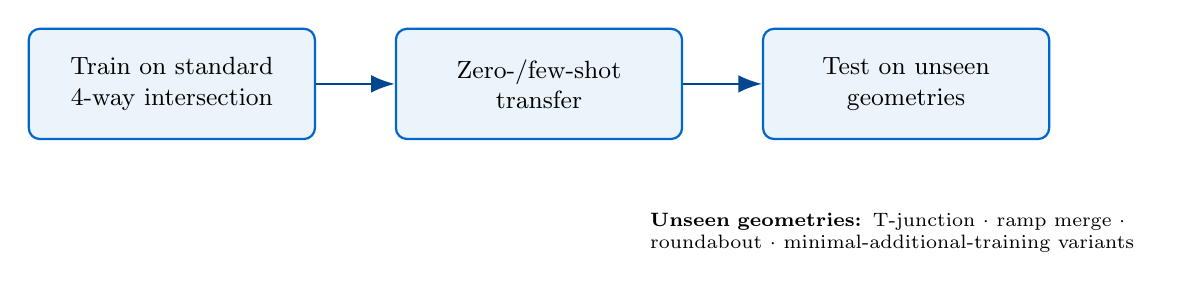
\begin{tikzpicture}[
        node distance=10mm and 10mm,
        every node/.style={font=\small},
        block/.style={draw=teal, thick, rounded corners, fill=teal!8, minimum height=1.4cm, text width=3.4cm, align=center},
        arrowstyle/.style={-{Latex[length=3mm]}, thick, teal!70!black}
    ]
        \node[block] (train) {Train on standard\\4-way intersection};
        \node[block, right=of train] (transfer) {Zero-/few-shot\\transfer};
        \node[block, right=of transfer] (test) {Test on unseen\\geometries};
        \draw[arrowstyle] (train) -- (transfer);
        \draw[arrowstyle] (transfer) -- (test);

        \node[below=8mm of test, text width=6.5cm, align=left, font=\scriptsize] (list) {
            \textbf{Unseen geometries:} T-junction $\cdot$ ramp merge $\cdot$ roundabout $\cdot$ minimal-additional-training variants
        };
    \end{tikzpicture}
    \vspace{6pt}
    \small This mirrors the finding in Klimke et al.\ \cite{klimke2022enhanced} that edge-aware graph representations generalize far better across intersection \emph{sizes} than vertex-only models --- suggesting a graph/relational state representation is a promising direction for our geometry-agnostic extension.
\end{frame}

\begin{frame}{Immediate Next Steps}
    \begin{enumerate}
        \item Complete the remaining 6/8 paper configurations (Mix-Attention ablation, replay-buffer segmentation)
        \item Build a T-junction and roundabout variant of the current \texttt{highway-env} scene
        \item Run zero-shot evaluation of the Project-3 Discrete SAC policy on these unseen geometries
        \item Investigate a graph-based or relational state encoding to support geometry transfer
        \item Quantify the sim-to-sim physics gap (highway-env vs.\ SUMO vs.\ the paper's environment) explicitly
    \end{enumerate}
\end{frame}

% (Conclusion slide)

\begin{frame}{Conclusion}
    \begin{itemize}
        \item Built and validated a full DRL training pipeline across three progressively harder milestones
        \item Achieved an exact, 1:1 architectural reproduction of Xiao et al.\ (2024) Discrete SAC \cite{xiao2024decision}, with matching or better safety/efficiency outcomes
        \item Traced result differences to simulator physics rather than implementation error --- a genuine scientific finding, not a failure
        \item Proposed a concrete, literature-grounded path toward \alert{geometry-agnostic, generalizable} intersection decision-making
    \end{itemize}
    \vspace{10pt}
    \centering \Large \textbf{Thank you --- Questions?}
\end{frame}

% =====================================================================
\section{GitHub Link and Individual Contribution}
% =====================================================================

\begin{frame}{GitHub Link and Individual Contribution}
    % [Template slide: Add GitHub repository link and individual contributions here]
\end{frame}

% =====================================================================
\appendix
\begin{frame}[allowframebreaks]{References}
    \tiny
    \bibliographystyle{plain}
    \bibliography{references}
\end{frame}

\end{document}
